\chapter{The QGIS software environment}

\pagestyle{fancy}
\fancyhf{}
\fancyhead[OC]{\leftmark}
\fancyhead[EC]{\rightmark}
%\renewcommand{\footrulewidth}{1pt}
\cfoot{\thepage}

%%%%%%%%%%%%%%%%%%%%%%%%%%%%%%%%%%%%%%%%%%%%%%%%%%%%%%%%%%%
%%%%%%%%%%%%%%%%%%%%%%%%%%%%%%%%%%%%%%%%%%%%%%%%%%%%%%%%%%%

%\section{First look at the QGIS software}

Open QGIS software (may need to open it in your program files manager).\\
The welcome window contains a number of panels.\\
When you have existing projects, you can open them from this welcome screen in the \emph{Recent Projects} panel.\\
To begin a new QGIS project, select \emph{new project} \begin{tabular}{@{}c@{}}
\includegraphics[width=3ex]{images/new_project_icon.png}\end{tabular}. (top left, highlighted in red) \\

\begin{figure}[!h]
	\centering
	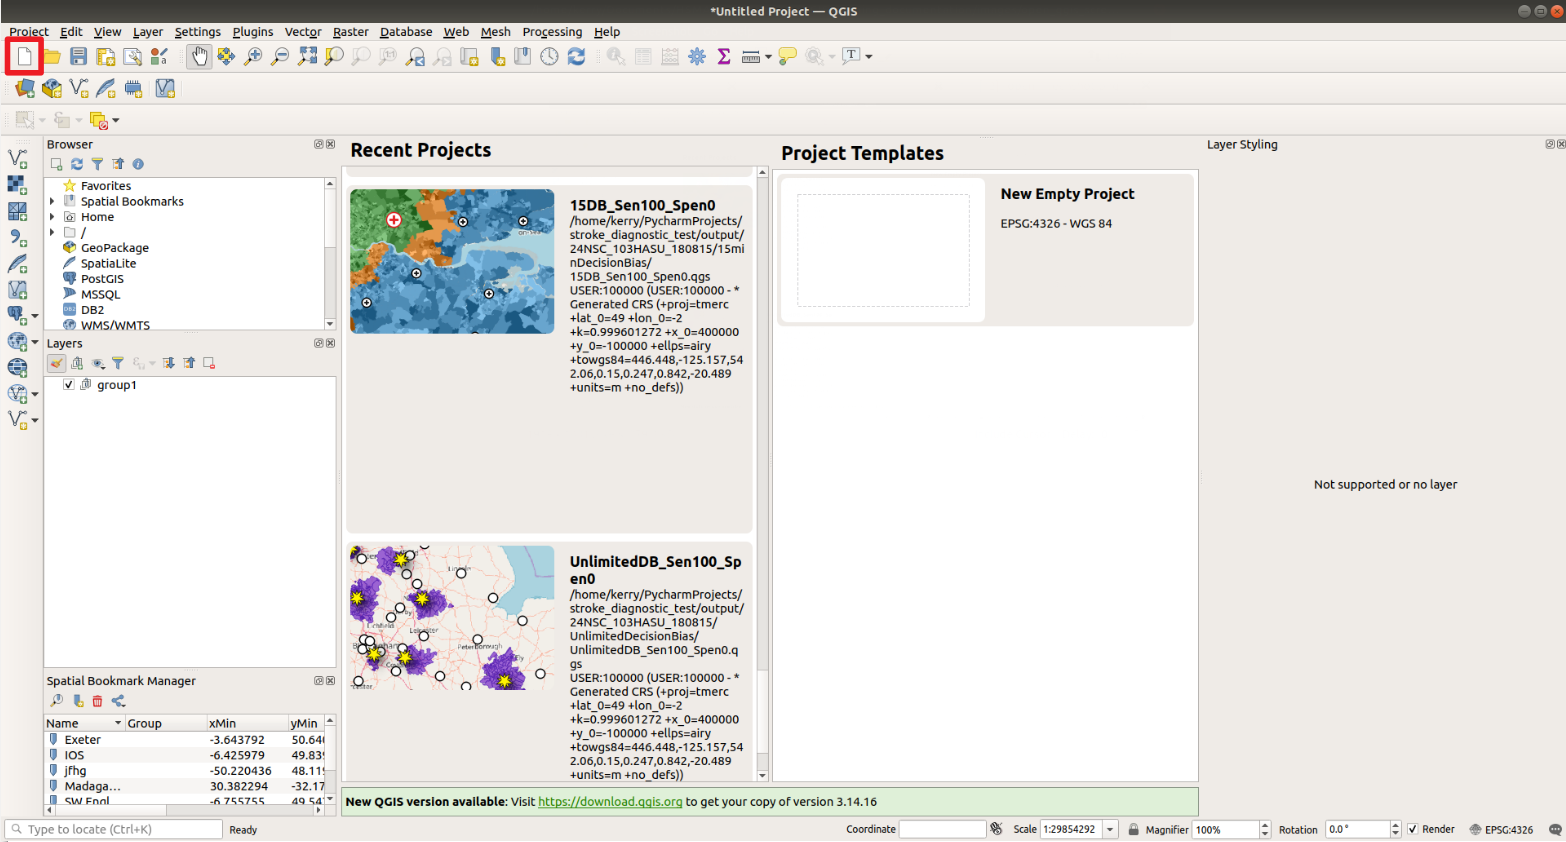
\includegraphics[width=0.62\textwidth]{images/open_qgis_screenshot_new_project.png}
	\caption{Screenshot of the QGIS welcome window}
	\label{ft_fig_firstfig3}
\end{figure}

Here is the QGIS project window, showing a new empty project.

%go to $C:\ProgramData\Microsoft\Windows\Start Menu\Programs\QGIS 2.18\QGIS Desktop 2.18.5$

\begin{figure}[!h]
	\centering
	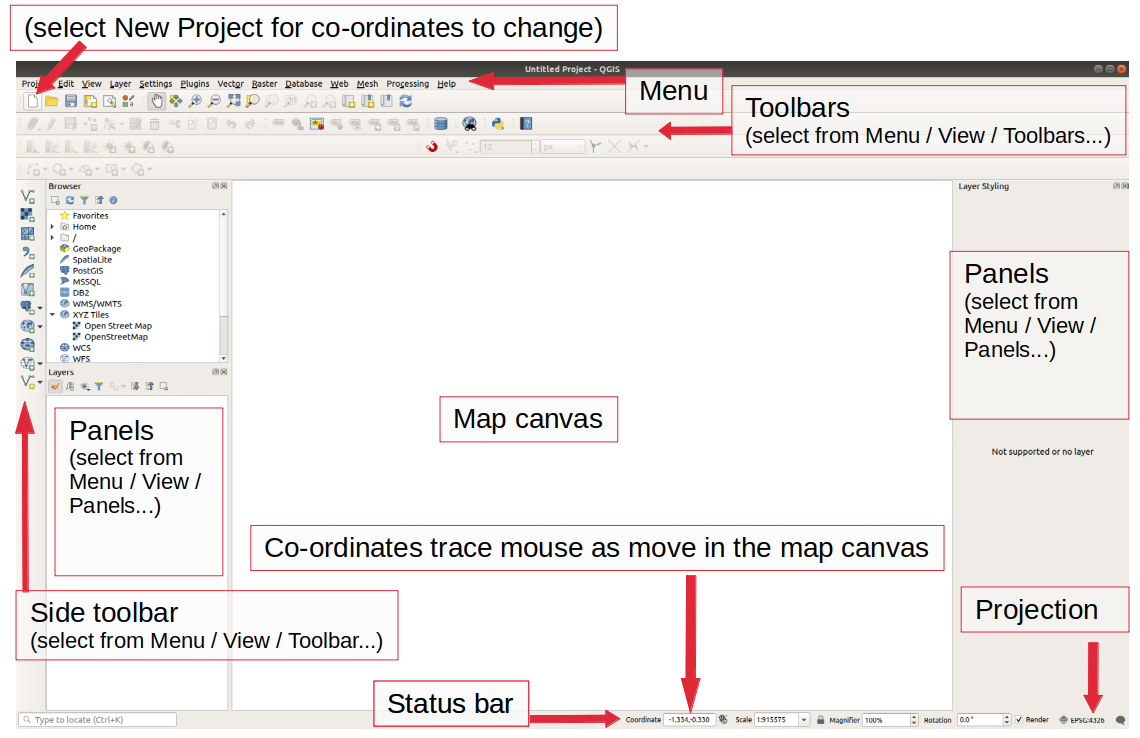
\includegraphics[width=0.62\textwidth]{images/full_window}
	\caption{Screenshot of the QGIS project window}
	\label{ft_fig_firstfig3}
\end{figure}

Become familiar with:
\begin{enumerate}[~~~1)]
	\item
	\textbf{Menu}
	\item
	\textbf{Map canvas}\\
	This is where the map is displayed
	\item
	\textbf{Status bar}\\
	Shows information about the current map view, and allows you to adjust the map scale and see the mouse cursor’s coordinates on the map (may need to select new project [blank page]). "Projection" contains the code for the current Coordinate Reference System (CRS) for the project (how software visually represents a 3D globe onto 2D screen).% CRS projections are methods to view 3D points on a 2D screen when the curvature of the Earth can often create a distorted image. WGS 84 is the reference system currently used by all GPS devices.
	
	\item
	\textbf{Toolbars}\\
	Give you easy access to frequently used tools (tools not visible in a toolbar, will remain accessible via the menus).\\
	Select which toolbars to have open from View $\rightarrow$ Toolbars menu\\
	Icons are disabled when they are not relevant (depending on the layers present in your project).\\
	Each icon has a useful tool tip.\\
	\\
	Useful toolbars for this tutorial are:	
	\begin{enumerate}
		\item
		Map navigation
		\item
		Data source manager
		\item
		Project
		\item
		Manage layers
		\item
		Attributes
	\end{enumerate}


%\begin{figure}[!h]
%	\centering
%	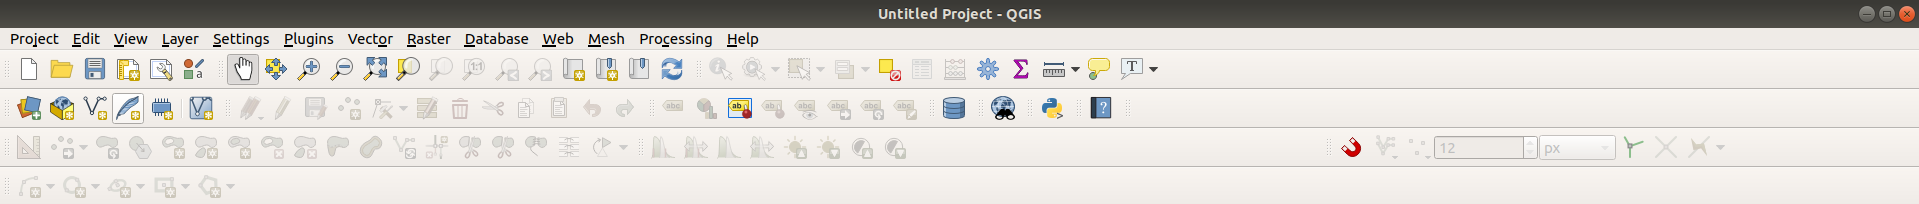
\includegraphics[width=1\textwidth]{images/top_toolbar}
%	\caption{Screenshot of all the icons in the toolbars at the top of the window}
%	\label{ft_fig_firstfig1}
%\end{figure}

%\begin{figure}[!h]
%	\centering
%	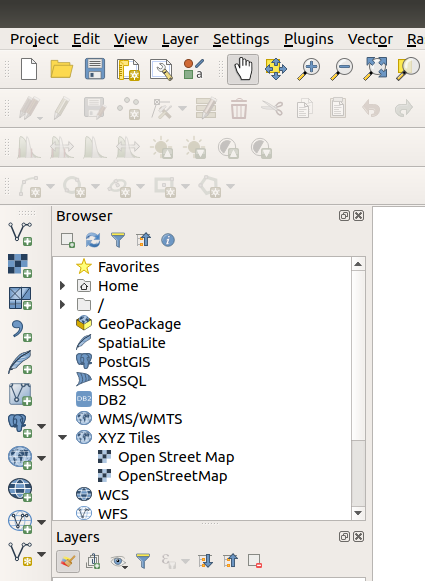
\includegraphics[width=0.21\textwidth]{images/side_toolbar}
%	\caption{Screenshot of all the icons in the toolbars at the side of the window}
%	\label{ft_fig_firstfig2}
%\end{figure}


	\item
	\textbf{Panels}\\ 
Select which to have open from View $\rightarrow$ Panels menu\\
If you use a command that requires a specific panel for the output, the relevant panel will automatically open.\\
Panels can be docked to the side of the window, share the docked space, be		full size using tabs, or float within the window.\\
\\
Useful panels for this tutorial are:	
\begin{enumerate}
	\item
Browser Panel\\
Navigate your file manager to open data files.
	\item
Layers\\
List of all the layers open in the project.  Expanding collapsed items provides you with more information on the layer’s current appearance. Right-clicking on a layer will give you a menu with lots of extra options. The order of the layers in this list determines the order that they are rendered on the map canvas.
	\item
Layer styling\\
Control the visual appearance of the layer on the map canvas (known as the symbology of a layer). \\

\end{enumerate}


\end{enumerate}

%\begin{figure}[!h]
%	\centering
%	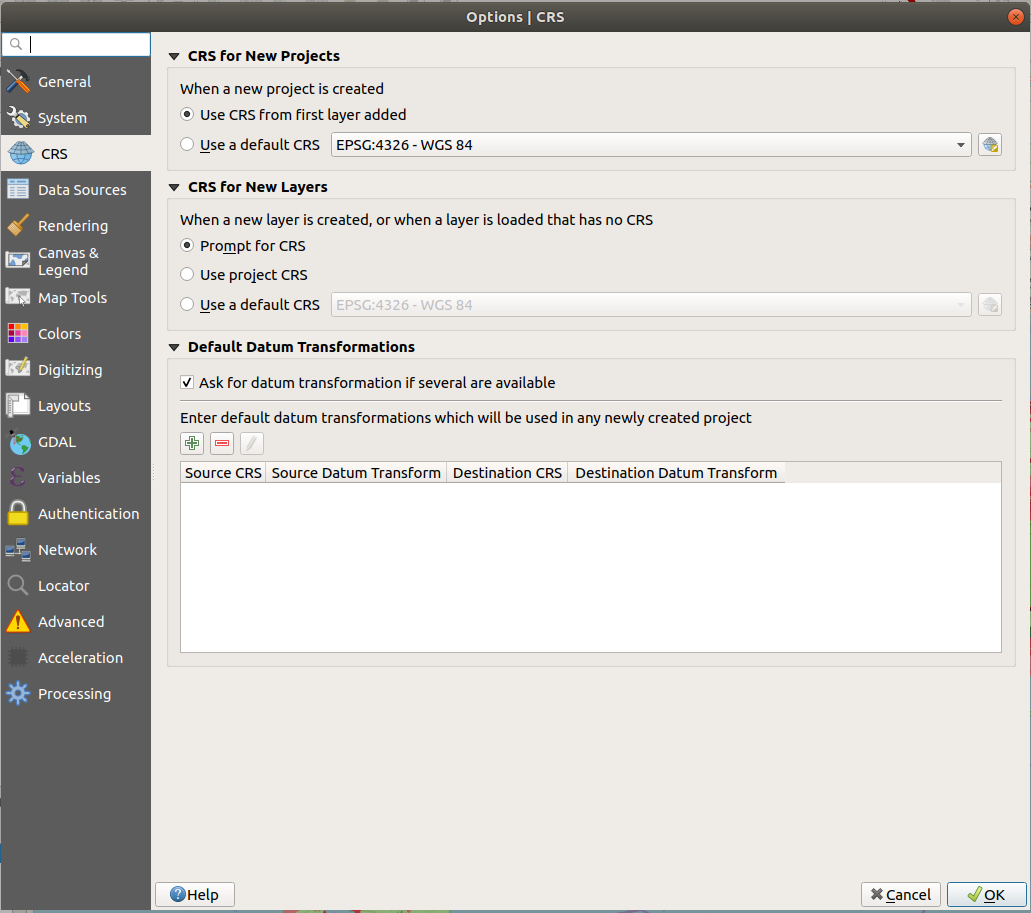
\includegraphics[width=0.8\textwidth]{images/settings_options_crs_window.png}
%	\caption{}
%	\label{ft_fig_firstfig3}
%\end{figure}